\begin{figure}
\begin{center}

\begin{subfigure}[b]{\columnwidth}
\centering
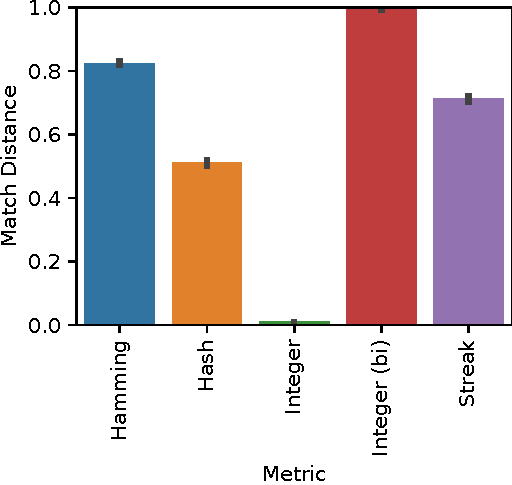
\includegraphics[width=\columnwidth]{sphere_reverse/bitweight=0dot5+seed=1+title=dimensionality_barplot+_data_hathash_hash=93f97a11cb443d35+_script_fullcat_hash=03ce1e318a24a109+ext=}
\caption{
Mean statistic values for each metric.
Error bars represent 95\% confidence intervals.
}
\label{fig:sphere_reverse_distnplot}
\end{subfigure}

\vspace{2ex}

\begin{subfigure}[b]{\columnwidth}
\centering
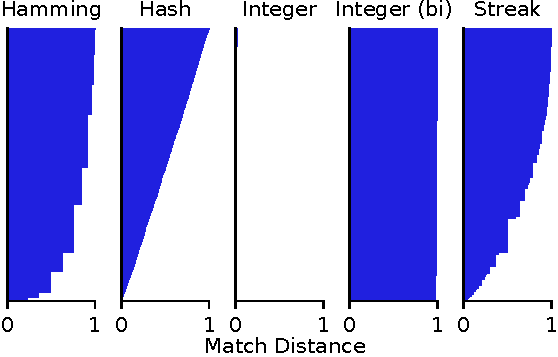
\includegraphics[width=\columnwidth]{sphere_reverse/bitweight=0dot5+seed=1+title=dimensionality_distnplot+_data_hathash_hash=93f97a11cb443d35+_script_fullcat_hash=03ce1e318a24a109+ext=}
\caption{
Statistic distribution, where each horizontal bar sliver represents one independent observation.
}
\label{fig:sphere_reverse_barplot}
\end{subfigure}

\caption{
Elasticity statistic measured as distances between two tags sampled, the first sampled from within 0.01 match distance of a third tag and the second sampled from outside 0.99 match distance of the third tag.
}
\label{fig:sphere_reverse}

\end{center}
\end{figure}
